%%%%%%%%%%%%%%%%%%%%%%%%%%%%%%%%%%%%%%%%%%%%%%%%%%%%%%
% A Beamer template for Ritsumeikan University       %
% Author: Ming-Hao Xu (Xu Minghao)                   %
% Date:   April 2022.                                %
% LPPL Licensed.                                     %
%%%%%%%%%%%%%%%%%%%%%%%%%%%%%%%%%%%%%%%%%%%%%%%%%%%%%%

\documentclass{beamer}
\usepackage{hyperref}

\usepackage[UTF8]{ctex}
\usepackage[T1]{fontenc}

% other packages
\usepackage{latexsym,amsmath,xcolor,multicol,booktabs,calligra}
\usepackage{graphicx,pstricks,listings,stackengine}
\usefonttheme[onlymath]{serif}

% dummy text; remove it when working on this template
\usepackage{lipsum}

\author{Ebola}
\title{计算几何1:点、向量、直线、凸包}
\institute{
    Institute of Mathematics, \\
    Zhejiang University.
}
\date{Jan, 2024}
\usepackage{Ritsumeikan}

% defs
\def\cmd#1{\texttt{\color{red}\footnotesize $\backslash$#1}}
\def\env#1{\texttt{\color{blue}\footnotesize #1}}
\definecolor{deepblue}{rgb}{0,0,0.5}
\definecolor{deepred}{rgb}{0.6,0,0}
\definecolor{deepgreen}{rgb}{0,0.5,0}
\definecolor{halfgray}{gray}{0.55}

\lstset{
    basicstyle=\ttfamily\tiny,
    keywordstyle=\bfseries\color{deepblue},
    emphstyle=\ttfamily\color{deepred},    % Custom highlighting style
    stringstyle=\color{deepgreen},
    numbers=left,
    numberstyle=\small\color{halfgray},
    rulesepcolor=\color{red!20!green!20!blue!20},
    frame=shadowbox,
}


\begin{document}

\begin{frame}
    \titlepage
\end{frame}

\begin{frame}
    \tableofcontents[sectionstyle=show,subsectionstyle=show/shaded/hide,subsubsectionstyle=show/shaded/hide]
\end{frame}

\section{二维几何基础}

\begin{frame}[fragile]{点与向量}
    二维平面上的任何一个点,可以用坐标 $(x,y)$ 表示。
    \vspace{1em}

    \pause
    向量是一个“具有方向和长度的箭头”,它不规定起点和终点。
    二维平面上的任何一个向量,也可以用坐标 $(x,y)$ 表示。
    \vspace{1em}

    \pause
    计算机存储点与向量没有区别,所以我们都可以用下面的结构体来存储。
\begin{lstlisting}[language=c++]
    struct Point{
        double x,y;
        Point(double x=0, double y=0): x(x), y(y) {}
    };
    #define Vector Point
    // 在计算机里,Vector 就是 Point,但为了从逻辑上区分,我们赋予它们不同的名字
\end{lstlisting}
\end{frame}


\begin{frame}[fragile]{浮点数比大小}
    \small
    浮点数是有限精度的,在运算过程中,难免会产生误差,
    相信大家深有被卡精度的体会。但是在计算几何中,我们
    经常需要判断浮点数的大小。\pause 这里我们引入如下的比较函数:
\begin{lstlisting}[language=c++]
    #define eps 1e-12
    int dcmp(double x)
    {
        if(fabs(x)<=eps) return 0;
        else if(x<0) return -1;
        else return 1;
    }
\end{lstlisting}
\end{frame}


\begin{frame}[fragile]{向量的基本运算}
    我们重载一些运算符来实现向量基本运算。
\begin{lstlisting}[language=c++]
    Vector operator + (Vector a, Vector b){return Vector(a.x+b.x, a.y+b.y);}
    Vector operator - (Vector a, Vector b){return Vector(a.x-b.x, a.y-b.y);}
    Vector operator - (Vector b){return Vector(-b.x, -b.y);}
    Vector operator * (Vector a, double x){return Vector(a.x*x, a.y*x);}
    Vector operator * (double x, Vector a){return Vector(a.x*x, a.y*x);}
    double Angle(Vector a){return atan2(a.y, a.x);}

    bool operator < (Point a, Point b){
        return a.x < b.x || (a.x == b.x && a.y < b.y);
    }
    bool operator == (Point a, Point b){
        return dcmp(a.x-b.x) == 0 && dcmp(a.y-b.y) == 0;
    }

    double Dot(Vector a, Vector b){return a.x*b.x + a.y*b.y;}
    double Length(Vector a){return sqrt(a.x*a.x + a.y*a.y);}
\end{lstlisting}
\end{frame}


\begin{frame}[fragile]{向量的叉乘}
    \small
    二维向量叉乘写作 $\mathbf{a}\times \mathbf{b}$,定义如下:
\begin{lstlisting}[language=c++]
    double Cross(Vector a,Vector b){return a.x*b.y - a.y*b.x;}
\end{lstlisting}

    \vspace{1em}\pause
    在几何中,叉乘是向量 $\mathbf{a}$ 与 $\mathbf{b}$ 构成的平行四边形的有向面积。
    如果 $\mathbf{b}$ 在 $\mathbf{a}$ 的\textbf{逆时针}方向,
    结果就是\textbf{正}的;逆时针方向就是负的;平行就是零。

    \begin{figure}
        \centering
        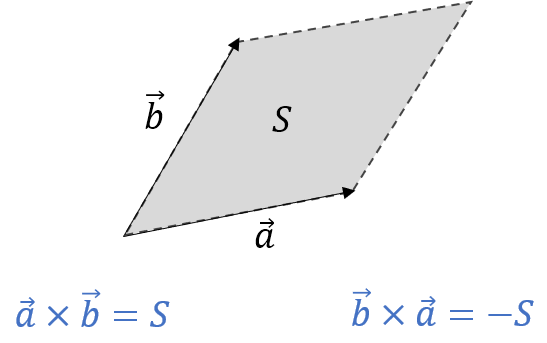
\includegraphics[width=0.4\textwidth]{pic/cross.png}
    \end{figure}

    \vspace{1em}\pause
    当向量坐标都是整数时,用叉乘判断向量相对位置没有精度误差!
\end{frame}


\begin{frame}[fragile]{叉乘的应用:将凸多边形的顶点按逆时针排序}
    给定凸 $n$ 边形的所有顶点,请将它们按逆时针排序,起点随意。

    (提示:使用 \verb|sort| 函数,考虑如何定义 \verb|cmp|)

    \vspace{1em}\pause
    先随意固定一个起点 $P_0$,$P_i$ 排在 $P_j$ 前面,当且仅当
    \begin{equation*}
        \overrightarrow{P_0P_i} \times \overrightarrow{P_0P_j} > 0.
    \end{equation*}

    \begin{figure}
        \centering
        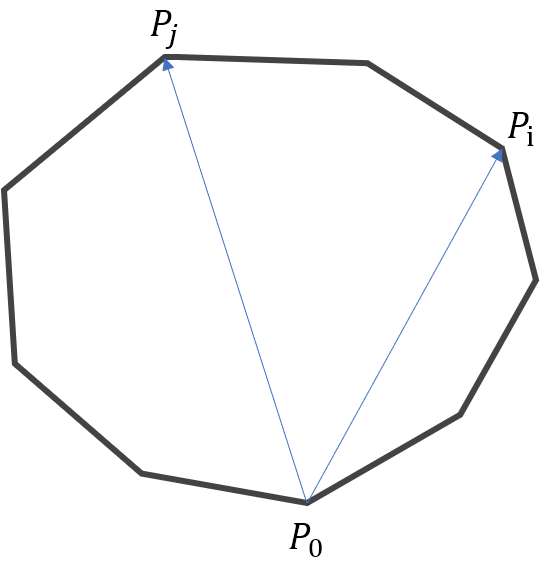
\includegraphics[width=0.4\textwidth]{pic/sort.png}
    \end{figure}
\end{frame}


\begin{frame}[fragile]{叉乘的应用:求凸多边形的面积}
    给定凸 $n$ 边形的所有顶点,它们已经按逆时针排好了序,求图形的面积。

    \vspace{1em}\pause
    \begin{figure}
        \centering
        
\includegraphics[width=0.3\textwidth]{pic/area.png}
    \end{figure}
    依次叉乘并累加即可。
\begin{lstlisting}[language=c++]
    double area = 0;
    for(int i = 2; i <= n-1; i++)
        area += 0.5 * cross(p[i]-p[1], p[i+1]-p[1]);
\end{lstlisting}
\end{frame}


\section{二维凸包}

\begin{frame}[fragile]{凸包}
    给定 $n$ 个点,你需要从中选取若干个点构成一个凸多边形,
    并且这个凸多边形包住了所有的点。

    \vspace{1em}
    模板题:P2742 [USACO5.1] 圈奶牛
\end{frame}

\begin{frame}[fragile]{凸包的拆分}
    我们通常将凸多边形拆分成两个部分:上凸壳和下凸壳。
    上下凸壳的分界点是凸多边形最左与最右的顶点。

    \begin{figure}
        \centering
        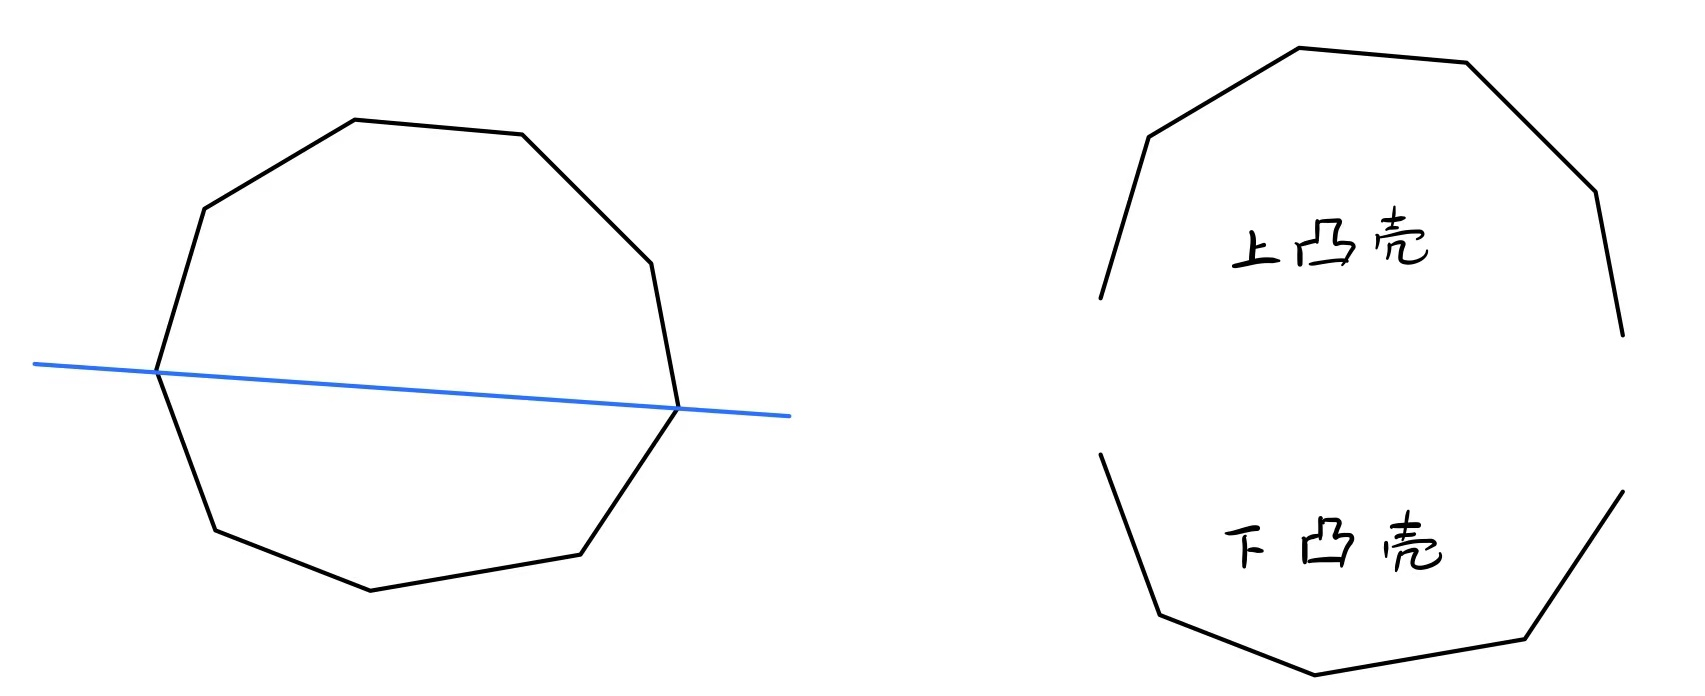
\includegraphics[width=0.7\textwidth]{pic/convex_split.jpg}
    \end{figure}
\end{frame}

\begin{frame}[fragile]{上凸壳的维护}
    \small
    维护上凸壳的一个基本想法是:用一个栈来存储当前上凸壳,
    然后考虑添加一个新的点。为了维护凸性,我们先弹出栈顶的一些元素,
    然后再将这个点加入。栈顶元素是否需要弹出可以根据叉乘的符号来判断。
    \pause
    \begin{figure}
        \centering
        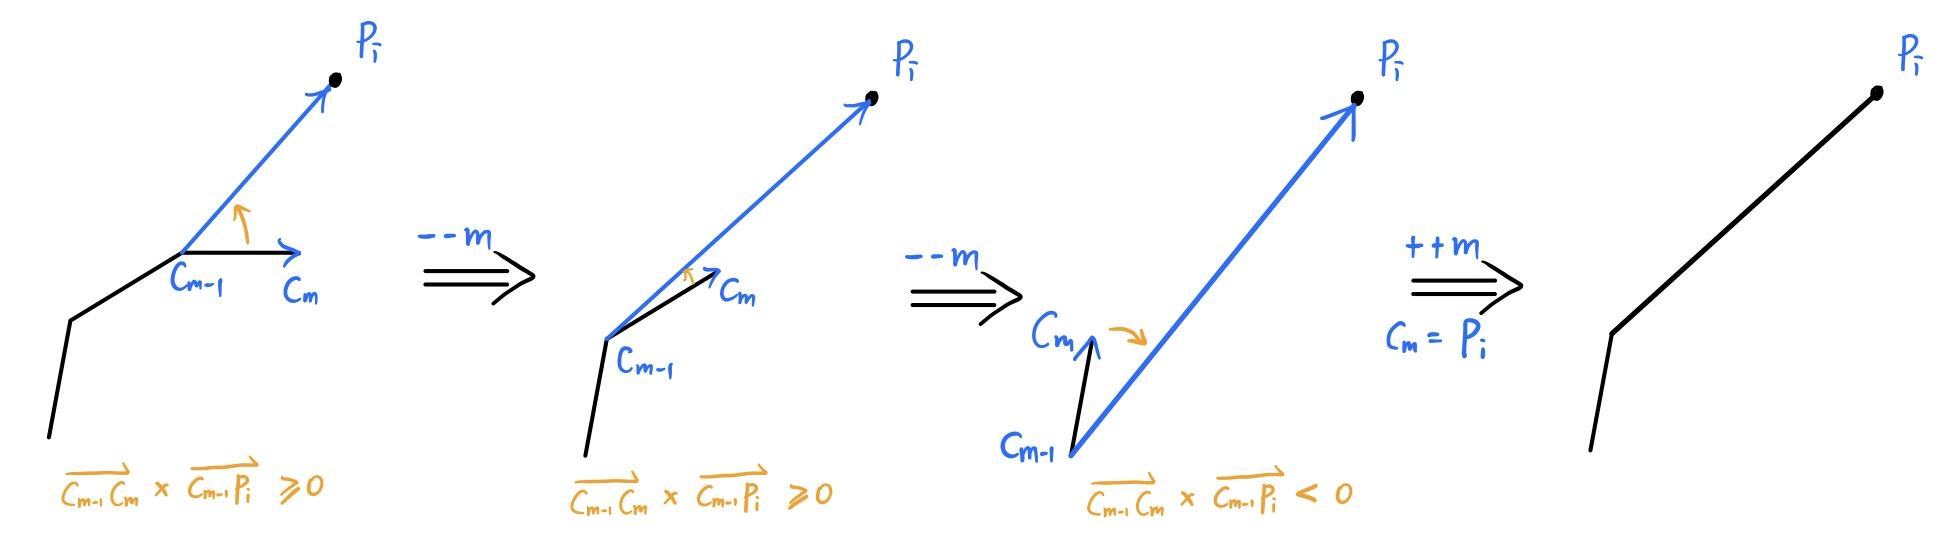
\includegraphics[width=\textwidth]{pic/convex_addpoint.jpg}
    \end{figure}
    \pause

    现在问题是:按什么样的顺序考虑新的点,才能保证正确地求出上凸壳?
\end{frame}

\begin{frame}[fragile]{点的加入顺序}
    \small
    答案是\textbf{从左到右、从下到上}。即将所有点按 $x$ 为第一关键字、
    $y$ 为第二关键字进行排序。这样为什么是对的?
    \vspace{1em}\pause

    其实我们只需要保证上凸壳上的点的访问顺序是从左到右,并且
    上凸壳最右边的点排在最后一个即可。
    对于不在上凸壳上的点,它们的顺序不重要,因为都会被弹出。
    显然,“从左到右、从下到上” 符合上述要求。
\end{frame}

\begin{frame}[fragile]{下凸壳的维护}
    \small
    维护下凸壳也很简单,只要把点的访问顺序倒过来即可,其余部分完全一样。
\end{frame}

\begin{frame}[fragile]{完整代码}
    \small
    \begin{lstlisting}[language=c++]
bool operator < (const Point &a,const Point &b){
    return a.x < b.x || (a.x == b.x && a.y < b.y);
}
int ConvexHull(Point a[],int n,Point b[]){
    sort(a+1, a+n+1);
    int m = 0;
    for(int i = 1; i <= n; i++){
        while(m > 1 && cross(b[m]-b[m-1], a[i]-b[m-1]) >= 0) --m;
        b[++m] = a[i];
    }
    int k = m;
    for(int i = n-1; i >= 1; i--){
        while(m > k && cross(b[m]-b[m-1], a[i]-b[m-1]) >= 0) --m;
        b[++m] = a[i];
    }
    return m-1;
}
    \end{lstlisting}

    \vspace{1em}\pause
    这样得到的凸包顶点是按顺时针方向排序的,如果要按逆时针方向排序,
    可以 \verb|reverse| 一下,或者直接把上面代码里的 \verb|>=| 改成 \verb|<=|。
\end{frame}

\begin{frame}{[SDOI2013] 保护出题人}
\footnotesize
僵尸从唯一一条笔直道路接近,你们需要在铭铭的房门前放置植物攻击僵尸,避免僵尸碰到房子。
\vspace{1em}

第一关,一只血量为$a_1$点的僵尸从距离房子$x_1$米处速接近,你们放置了攻击力为$y_1$点/秒的植物进行防御;第二关,在上一关基础上,僵尸队列排头增加一只血量为$a_2$点的僵尸,与后一只僵尸距离$d$米,从距离房$x_2$米处匀速接近,你们重新放置攻击力为$y_2$点/秒的植物;……;第$n$关,僵尸队列共有$n$只僵尸,相邻两只僵尸距离$d$米,排头僵尸血量为$a_n$点,排第二的 僵尸血量$a_{n-1}$,以此类推,排头僵尸从距离房子$x_n$米处匀速接近,其余僵尸跟随排头同时接近,你们重新放置攻击力为$y_n$点/秒的植物。

\vspace{1em}
每只僵尸直线移动速度均为$1$米/秒,由于植物射击速度远大于僵尸移动速度,可忽略植物子弹在空中的时间。所有僵尸同时出现并接近,因此当一只僵尸死亡后,下一只僵尸立刻开始受到植物子弹的伤害。

\vspace{1em}
游戏得分取决于你们放置的植物攻击力的总和$\sum \limits _{i=1} ^{n} y_i$,和越小分数越高,为了追求分数上界,你们每关都要放置攻击力尽量小的植物。
\end{frame}

\begin{frame}{[SDOI2013] 保护出题人}
    \footnotesize
    \begin{figure}[H]
        \centering
        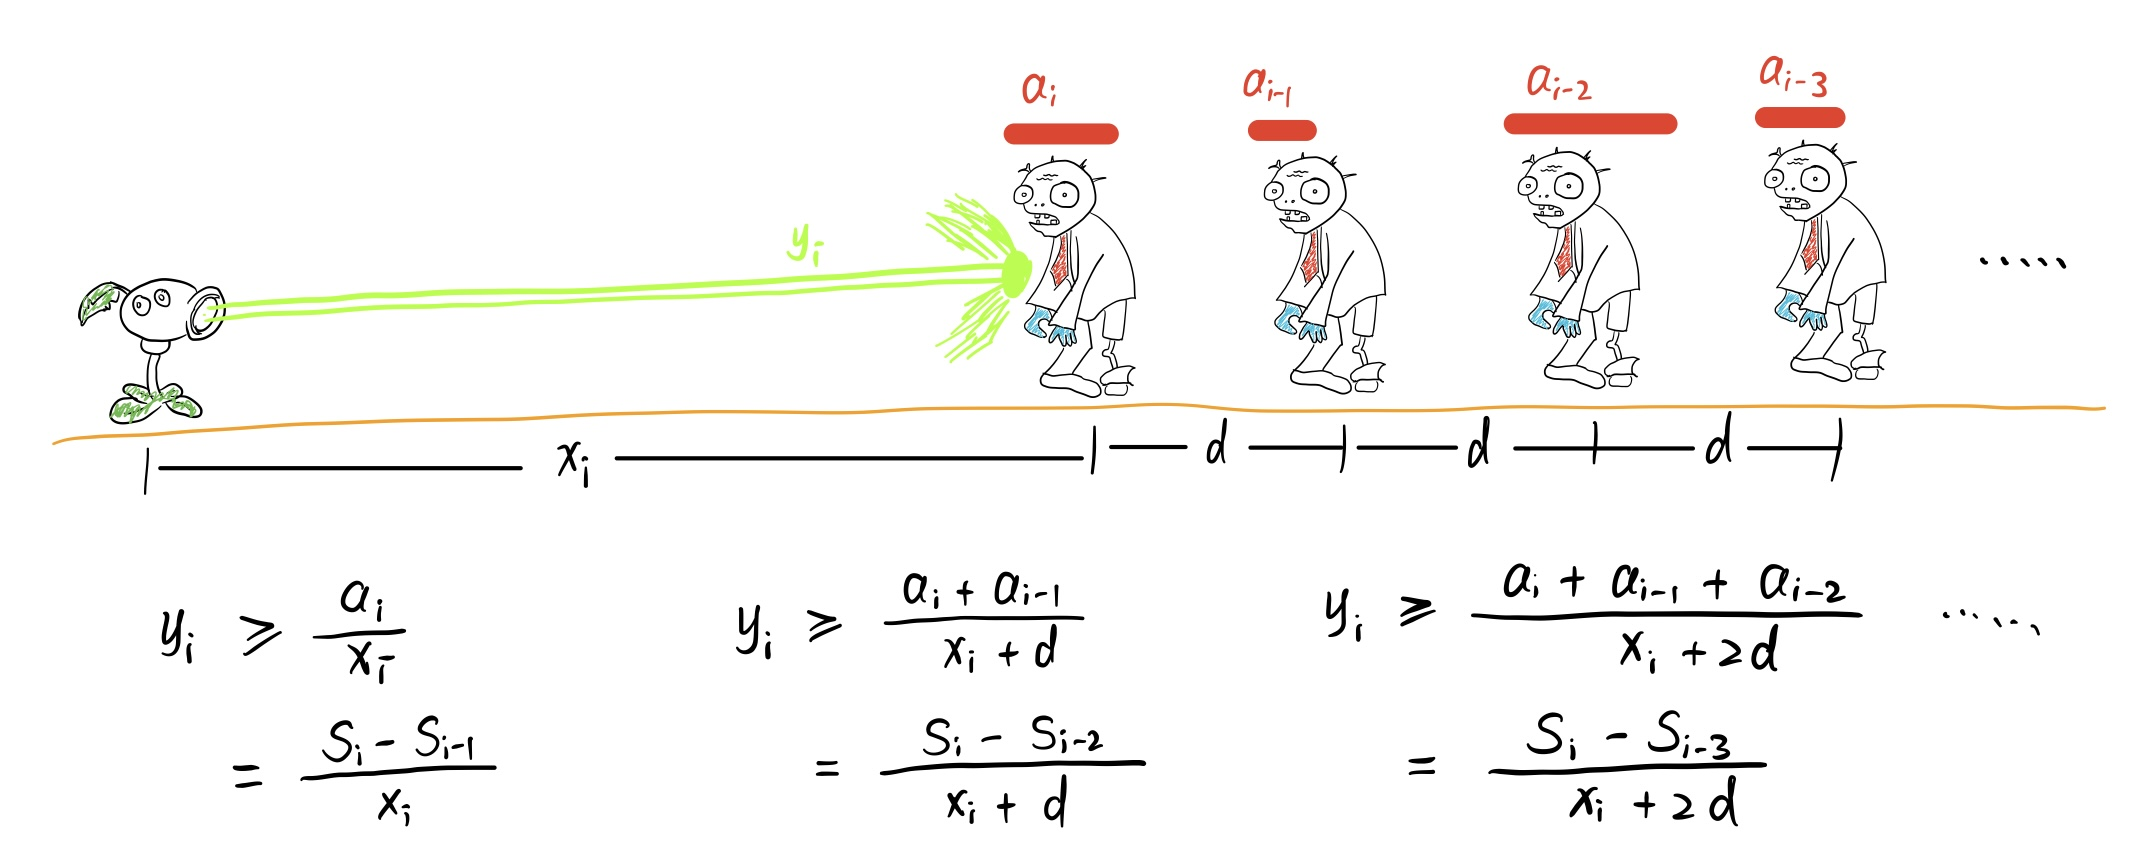
\includegraphics[width=\textwidth]{pic/sdoi2013.jpg}
    \end{figure}
    图中 $S_i$ 表示 $a_i$ 的前缀和。试着写出 $y_i$ 的表达式:
    \pause
    \begin{equation}
        y_i=\max_{1\leq j\leq i} \frac{S_i-S_{j-1}}{(x_i+i*d)-j*d}.
    \end{equation}
    也就是点 $(x_i+i*d,S_i)$ 与 $(j*d,S_{j-1})$ 的连线的斜率。
\end{frame}

\begin{frame}{[SDOI2013] 保护出题人}
    \footnotesize
    现在我们可以写出算法的大致框架:

    \begin{enumerate}
        \item 将 $(i*d, S_{i-1})$ 加入点集 $P$;
        \item 在点集 $P$ 中寻找与 $(x_i+i*d,S_i)$ 连线的最大斜率 $k$;
        \item $ans+=k$;
        \item $i++$,然后重复第一步。
    \end{enumerate}

    关键在于第二步如何优化。
    \pause
    斜率最大的点一定在 $P$ 的\textbf{下凸壳}中!为什么?
    \pause
    \begin{figure}[H]
        \centering
        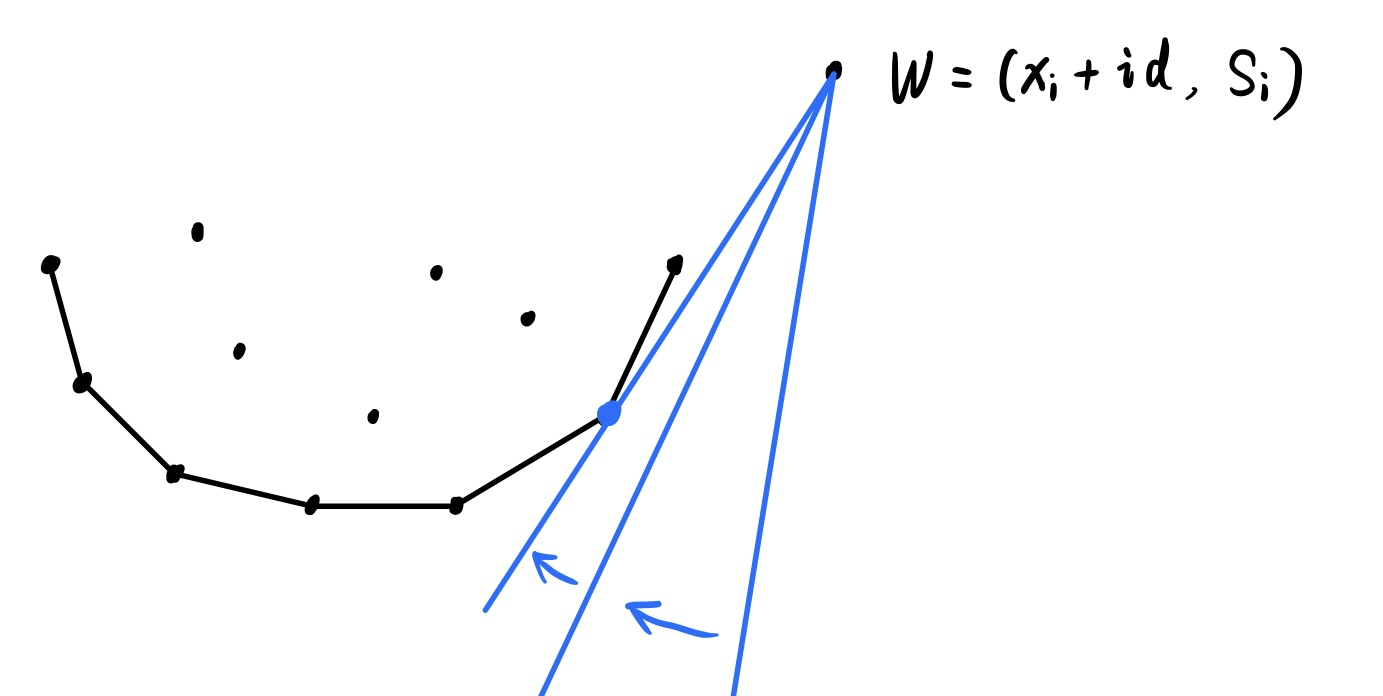
\includegraphics[width=0.6\textwidth]{pic/sdoi2013-2.jpg}
    \end{figure}
    如图所示,从 $W$ 向下引一条射线,并逆时针旋转,
    碰到的第一个点一定是下凸壳的某个顶点。
\end{frame}

\begin{frame}[fragile]{[SDOI2013] 保护出题人}
    \footnotesize
    那么我们只需要维护 $P$ 的下凸壳就行了,
    因为加入新点的顺序自然地就是从左到右,
    所以每次加入一个新点,
    用凸包算法里的 \verb|while| 循环维护一下就好了。

    怎么快速求下凸壳里的最大斜率?

    \vspace{1em}\pause
    我们记下凸壳顶点为 $P_1,...,P_m$,
    容易发现 $k_{WP_1},...,k_{WP_m}$ 是先增后减的,
    所以三分即可。
\end{frame}

\begin{frame}[fragile]{[SDOI2014] 向量集}
    \small
    维护一个向量集合,在线支持以下操作:

    \begin{itemize}
    \item \verb|A x y|($|x|,|y| \le 10^8$):加入向量 $(x,y)$;
    \item \verb|Q x y l r|($|x|,|y| \le 10^8$,$1 \le l \le r \le t$,其中 $t$ 为已经加入的向量个数):询问第 $l$ 个到第 $r$ 个加入的向量与向量 $(x,y)$ 的点积的最大值。
    \end{itemize}

    集合初始时为空。
\end{frame}

\begin{frame}[fragile]{[SDOI2014] 向量集}
    \small
    我们记 $P_i$ 是第 $i$ 个加入的向量的坐标,
    并且我们把 $P_i$ 视为一个点。
    我们记 $Q$ 是询问时输入的向量坐标,
    同样的我们把 $Q$ 视为一个点。
    那么我们需要最大化:
    \begin{equation}
        \overrightarrow{OP_i}\cdot \overrightarrow{OQ},\quad i\in[l,r].
    \end{equation}

    \pause 这等价于最大化:
    \begin{equation}
        \frac{\overrightarrow{OP_i}\cdot \overrightarrow{OQ}}{|\overrightarrow{OQ}|} ,\quad i\in[l,r].
    \end{equation}

    而这就是线段 $OP_i$ 在直线 $l_{OQ}$ 上的投影长度。
    投影长度最大的点一定位于……?

    \pause $P_l,...,P_r$ 的 \textbf{凸包}!(包括上凸壳和下凸壳,因为坐标可能有负的)
\end{frame}

\begin{frame}[fragile]{[SDOI2014] 向量集}
    \small
    维护一个线段树即可,每个节点存储对应区间的上凸壳、下凸壳。
    询问时直接在线段树节点对应的区间上分别查询,然后取最大值即可。
    现在问题是如何合并左右儿子的上(下)凸壳?

    \vspace{1em}\pause
    拿出来 \verb|sort| 一遍显然是不好的,会变成两个 log。
    但是左右儿子的上(下)凸壳各自是排好序的,所以我们可以\textbf{二路归并}。

    \vspace{1em}\pause
    注意,合并过程在 \verb|insert| 过程中发生,
    且只有当 $r==i$ 时才合并该节点的左右儿子的上(下)凸壳
    (这是因为当 $i<r$ 时,询问操作并不会访问到这个节点的凸包),
    这样可以保证复杂度是正确的。
\end{frame}

\begin{frame}{[CERC2014] Mountainous landscape}
    \small
    给定平面内一个由点依次连接起来形成的折线 $P_1,P_2,\cdots,P_n$,保证 $x$ 坐标递增。
    
    对于折线上的所有线段,找到最小的 $j>i$,使得存在一个在 $P_jP_{j+1}$ 上的点可以被 $P_iP_{i+1}$ 上的任何一个点看到,也就是\textbf{严格}在射线 $P_iP_{i+1}$ 上方。若没有,输出 $0$.
    
    多组数据。
    
    $2\le n\le 10^5$,坐标均在 $10^9$ 以内。
\end{frame}

\begin{frame}{[CERC2014] Mountainous landscape}
    \small
    仍然考虑用线段树维护上凸壳,这里我们可以提前建树。
    然后在线段树上二分:
    \begin{itemize}
    \pause \item 若左儿子与 $[i+1,n]$ 有交,且左儿子的凸包与射线 $P_{i}P_{i+1}$ 有交,
    那么往左走;
    \pause \item 若右儿子的凸包与射线 $P_{i}P_{i+1}$ 有交,
    那么往右走;
    \pause \item 否则,说明答案不存在。
    \end{itemize}

    现在的问题是如何快速判断一个凸包与射线是否相交?

    \pause
    凸包上边的斜率是递减的,可以二分找到第一个斜率 $\leq k_{P_{i}P_{i+1}}$
    的边,这条边的左端点是最有可能位于射线 $P_{i}P_{i+1}$ 上方的点,判断即可。
\end{frame}

\begin{frame}{[HAOI2011] 防线修建(动态凸包)}
    \small
    给定平面内 $m$ 个点,你需要支持如下操作:
    \begin{itemize}
        \item 询问上凸壳所有边的长度之和;
        \item 删除一个点。
    \end{itemize}
    $m\leq 10^5$,坐标都是 $[0,10^4]$ 中的整数。
\end{frame}

\begin{frame}{[HAOI2011] 防线修建(动态凸包)}
    \footnotesize
    先把所有操作离线,然后倒过来处理操作,即:
    先把没被删掉的点的凸包求好,
    然后按删除的顺序反过来把点依次加回去。

    \pause\vspace{.5em}
    问题是新加的点并不在已有凸壳的右侧,怎么办?

    \pause\vspace{.5em}
    把凸壳视为两部分,一部分在新加点左侧,一部分在新加点右侧,
    我们需要二分找到分界点。
    \pause 对于左侧,按照维护上凸壳的方式弹出一些点;
    对于右侧,也按照类似的方式弹出一些点;最后加入新点。

    \begin{figure}[H]
        \centering
        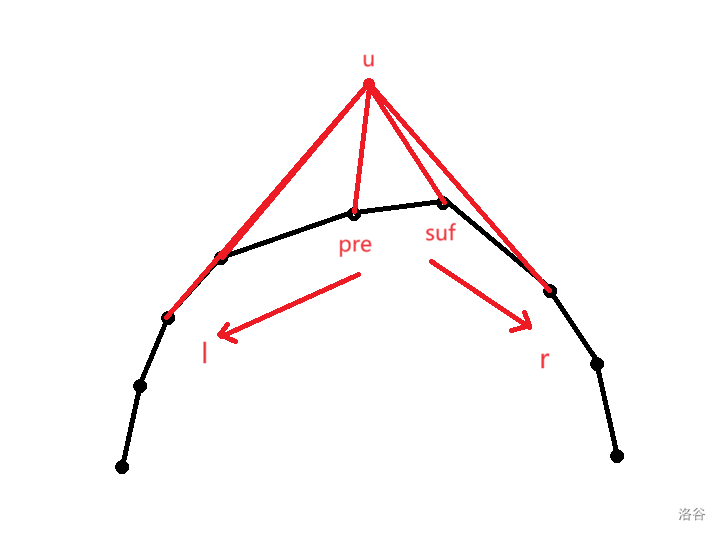
\includegraphics[width=0.5\textwidth]{pic/haoi2011.png}
    \end{figure}

    \pause 需要一个可以插入点、删除任意点、保序的结构,用 set 即可。

\end{frame}

\section{点与直线}

\begin{frame}[fragile]{判断点与线段的位置关系}
    \small
    考虑如何判断点 $P$ 是否在线段 $AB$ 上。
    (不要去想斜率,因为算斜率会引入精度误差,而且斜率无穷大时还要特判)

    \vspace{1em}\pause
    \begin{align}
        \overrightarrow{AB}\times  \overrightarrow{AP}&=0\\
        \overrightarrow{PA}\cdot  \overrightarrow{PB}&<0
    \end{align}

    \vspace{1em}\pause
    \begin{lstlisting}[language=c++]
bool PointInSegment(Point p, Point a, Point b){
    return Cross(b-p, a-p) == 0 && Dot(b-p, a-p) < 0;
}
    \end{lstlisting}

    \vspace{1em}\pause
    其实通过 $\overrightarrow{AB}\times  \overrightarrow{AP}$
    的符号,我们还可以判断 $P$ 的方位:大于零时,在 $\overrightarrow{AB}$
    左侧;小于零时,在 $\overrightarrow{AB}$ 右侧。
\end{frame}

\begin{frame}[fragile]{判断两条线段是否相交}
    \small
    考虑如何判断线段 $AB$ 与 线段 $CD$ 是否相交。

    \vspace{1em}\pause
    两条线段相交当且仅当下面两个条件同时满足:
    \begin{itemize}
        \item $A,B$ 在 $l_{CD}$ 的两侧;
        \item $C,D$ 在 $l_{AB}$ 的两侧。
    \end{itemize}

    \vspace{1em}\pause
    \begin{lstlisting}[language=c++]
bool SegmentProperIntersection(Point a1, Point a2, Point b1, Point b2)
{
    long long c1 = Cross(b1-a1, a2-a1);
    long long c2 = Cross(b2-a1, a2-a1);
    long long c3 = Cross(a1-b1, b2-b1);
    long long c4 = Cross(a2-b1, b2-b1);
    return c1*c2 < 0 && c3 * c4 < 0;
}
    \end{lstlisting}
\end{frame}

\begin{frame}[fragile]{判断点是否在凸多边形内部}
    \small
    考虑如何判断点 $P$ 是否在凸多边形的内部(或者边界上)。
    其中凸多边形的顶点 $A_1,...,A_n$ 按照逆时针顺序给出。

    \vspace{1em}\pause
    判断是否在边界上很简单,用刚刚的 \verb|PointInSegment| 即可。

    \vspace{1em}\pause
    判断是否在内部只需检查以下条件:
    \begin{equation}
        \overrightarrow{A_iA_{i+1}}\times  \overrightarrow{A_iP}>0
    \end{equation}
    对所有的 $i$ 都成立(当 $i=n$ 时, $i+1$ 用 $1$ 代替)。
\end{frame}

\begin{frame}{判断点是否在任意多边形内部}
    \small
    考虑如何判断点 $P$ 是否在任意多边形的内部(或者边界上)。
    其中多边形的顶点 $A_1,...,A_n$ 按照逆时针顺序给出。

    \vspace{1em}\pause
    射线法:从 $P$ 向任意方向引出一条射线,如果射线与多边形边界
    有奇数个交点,说明在内部,否则就在外部。
    (写程序时,一般取水平向右的射线)
\end{frame}

\begin{frame}[fragile]{判断点是否在任意多边形内部}
    \small
    \begin{lstlisting}[language=c++]
bool PointInPolygon(Point p,Point* res,int cnt)
{
    int wn=0;
    for (int i=0;i<cnt;i++)
    {
        if(res[i]==p||res[(i+1)%cnt]==p||PointInSegment(p,res[i],res[(i+1)%cnt]))
            return 1;
        // 射线法
        int k=Cross(res[(i+1)%cnt]-res[i],p-res[i]);
        int d1=res[i].y-p.y;
        int d2=res[(i+1)%cnt].y-p.y;
        if(k>0&&d1<=0&&d2>0) wn++;
        if(k<0&&d2<=0&&d1>0) wn--;
    }
    if(wn) return 1;
    return 0;
}
    \end{lstlisting}
\end{frame}

\begin{frame}{[UVA10256] 判断两个点集能否分离}
    \small
    给定两组点集(每组最多 500 个点),问是否存在一条直线能将它们分离?

    \vspace{1em}\pause
    分别求凸包,转换为两个凸包是否相交的判定问题。

    \vspace{1em}\pause
    枚举凸包 $A$ 的所有顶点,判断是否在凸包 $B$ 内部,
    然后反过来再来一次。(这样是否充分?)

    \pause
    \begin{figure}[H]
        \centering
        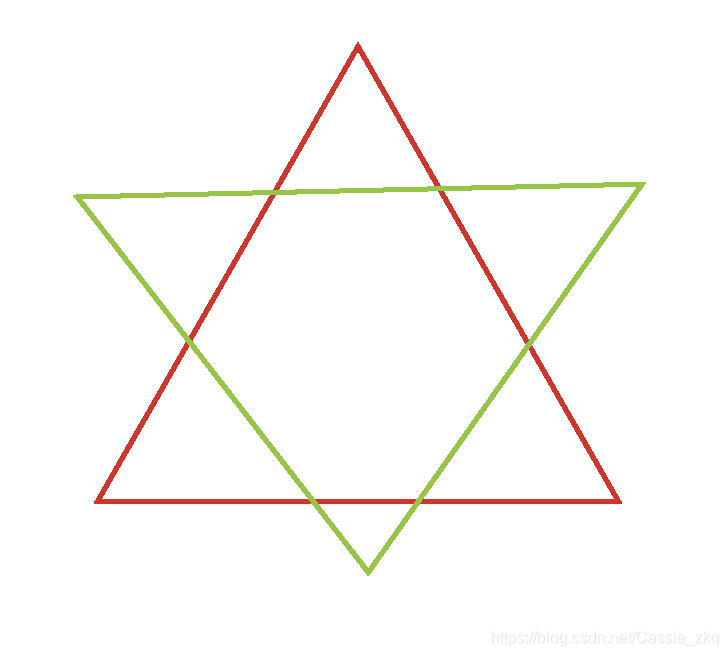
\includegraphics[width=0.3\textwidth]{pic/convexInsect.png}
    \end{figure}

    显然不充分,所以还要枚举凸包 $A$ 与凸包 $B$ 的所有边,
    然后调用线段相交的判定方法。
\end{frame}

\begin{frame}
    \begin{center}
        {\Huge\calligra Thank You}
    \end{center}
\end{frame}

\end{document}